\section{Switched Inductor}\label{ch:SIBC}
The Switched Inductor Boost Converter (SIBC) is a small alternation to the Conventional Boost Converter mentioned in Chapter \ref{ch:CBC}.
It only adds passive components to an already known topology,
which means the same switching scheme can be used.
\subsection{Additions from Conventional BC}
In the SIBC,
the single inductor from the Conventional BC gets replaced by two inductors and three diodes,
connected as shown in Figure \ref{fig:SwitchedInductor}.

\begin{figure} [H]
   \centering
   \includegraphics[width=0.6\textwidth]{figures/bSwitchedInductor/switched_inductor.pdf}
    \caption{Switched inductor boost converter circuit}
	\label{fig:SwitchedInductor}
\end{figure}


With this configuration,
the inductors form two different topologies during the ON and OFF states. By reversing the biasing of the diodes the inductors are connected in parallel during ON state and series during OFF state.  \todo[color=c04b]{refer to figure maybe} 


\subsection{Switching States}
The same switching scheme as for the Conventional BC can be used,
as mentioned earlier. We assume the sizes of all capacitors is equal.
The equivalent circuits during the on and off stages are shown in Figure \ref{fig:SI_States}.

\begin{figure}[H]%
    \centering
    \subfloat[Switch ON\label{SI_ON}]
    {{\includegraphics[width=0.45\textwidth]{figures/bSwitchedInductor/switched_inductorON.pdf} }}%
    \qquad
    \subfloat[Switch OFF\label{SI_OFF}]{{\includegraphics[width=0.45\textwidth]{figures/bSwitchedInductor/switched_inductorOFF.pdf} }}%  
    \caption{Switching states of the SIBC}%
     \label{fig:SI_States}% 
\end{figure}

\subsubsection{ON State}
While the switch is ON, diodes D\textsubscript{1} and D\textsubscript{2} are forward biased and diode D\textsubscript{3} is reverse biased.
This constructs a parallel conection between the inductors, as seen in Figure \ref{SI_ON}.
\\*
In this case, we can use KVL to build the eqation: 

\begin{equation}
	V_L=V_{in}
	\label{eq:SI_KVL_ON}
\end{equation}

\subsubsection{OFF State}
While the switch is OFF, the complete opposite happens, where only D\textsubscript{2} remains forward biased and forms a series connections between the inductors (shown on Figure \ref{SI_OFF}).
In a configuration like this we can assume equal split of the pottential across the inductors and using KVL construct the equation:
\begin{equation}
	V_{in}-2V_L-V_o=0
	\label{eq:SI_KVL_OFF}
\end{equation}\\
Subsequetially reformed as:
\begin{equation}
	V_L=\frac{V_{in} - V_o}{2}
	\label{eq:SI_KVL_OFF2}
\end{equation}
Reforming the Inductor voltage-second balance (Explained in Sections \ref{sec:convertionRatio} for the current topology, we get the following relationship:

\begin{equation}
	V_{L(ON)}D+V_{L(OFF)}(1-D)=0
	\label{eq:SI_IVSB}
\end{equation}
Substituting the already derived expressions for V\textsubscript{L}:

\begin{equation}
	V_{in}D+\frac{V_{in} - V_o}{2}(1-D)=0
	\label{eq:SI_IVSB2}
\end{equation}
Subsequenlty the input/output relationship can be stated as:

\begin{equation}
	\frac{V_o}{V_{in}} = \frac{1+D}{1-D}
	\label{eq:SI_VO_VIN}
\end{equation}
This shows the superior boost ration of the SIBC over the conventional boost converter. 

\subsection{Simulation results}

To confirm the calculations, the circuit was simulated in SIMULINK, using the following parameters: 

\begin{table}[H]
\begin{center}
\caption {Simulation parameters for SIBC} \label{tab:SI} 
\begin{tabular}{|l|l|}
\cline{1-2}
\textbf{Parameter} & \textbf{Value}  \\ \cline{1-2}
Input Voltage $V_{in}$          &      10V   \\ \cline{1-2}
Load(R)   & 225$\Omega$           \\ \cline{1-2}
Capacitance(C)          &       220$\mu$F     \\ \cline{1-2}
Inductance(L)          &      150$\mu$F      \\ \cline{1-2}
Duty cycle(D)          &     0.6       \\ \cline{1-2}
Switching Frequency($F_S$)          &      50KhZ      \\ \cline{1-2}
\end{tabular}
\end{center}
\end{table}

The whole topology was modelled within the software, with the listed values (Model can be seen on Figure.\ref{fig:Model_SI}). Components were assumed ideal, internal resistance and voltage drops are neglected during the simulation. 

\begin{figure} [H]
   \centering
   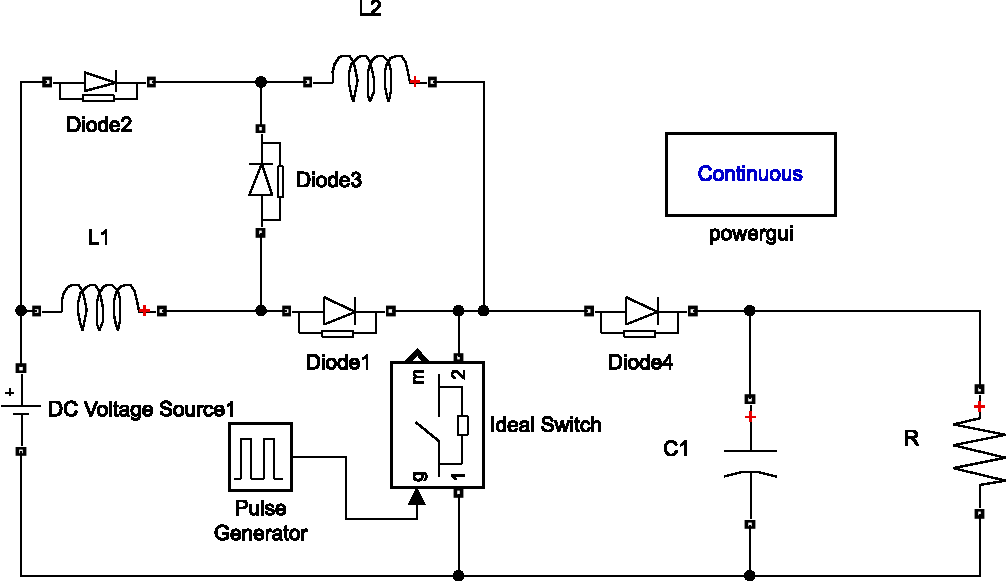
\includegraphics[width=0.8\textwidth]{figures/bSwitchedInductor/Model_SI.pdf}
    \caption{Switched inductor boost converter SIMULINK Model}
	\label{fig:Model_SI}
\end{figure}

Expected output voltage $V_O$ is calculated using Eq. \ref{eq:SI_VO_VIN} to calculate the gain and multiplying it by $V_in$: 
\begin{equation}
	{V_o}= \frac{1+0.6}{1-0.6}10=40V
	\label{eq:Simulation_SI}
\end{equation}

The simulation results show the system output is as expected, as observed on Figure. \ref{fig:Simulation_SI}. Voltage levels converge at 40 V. The overshoot and ripple can be improved on, but this is not within the scope of this project. 


\begin{figure} [H]
   \centering
   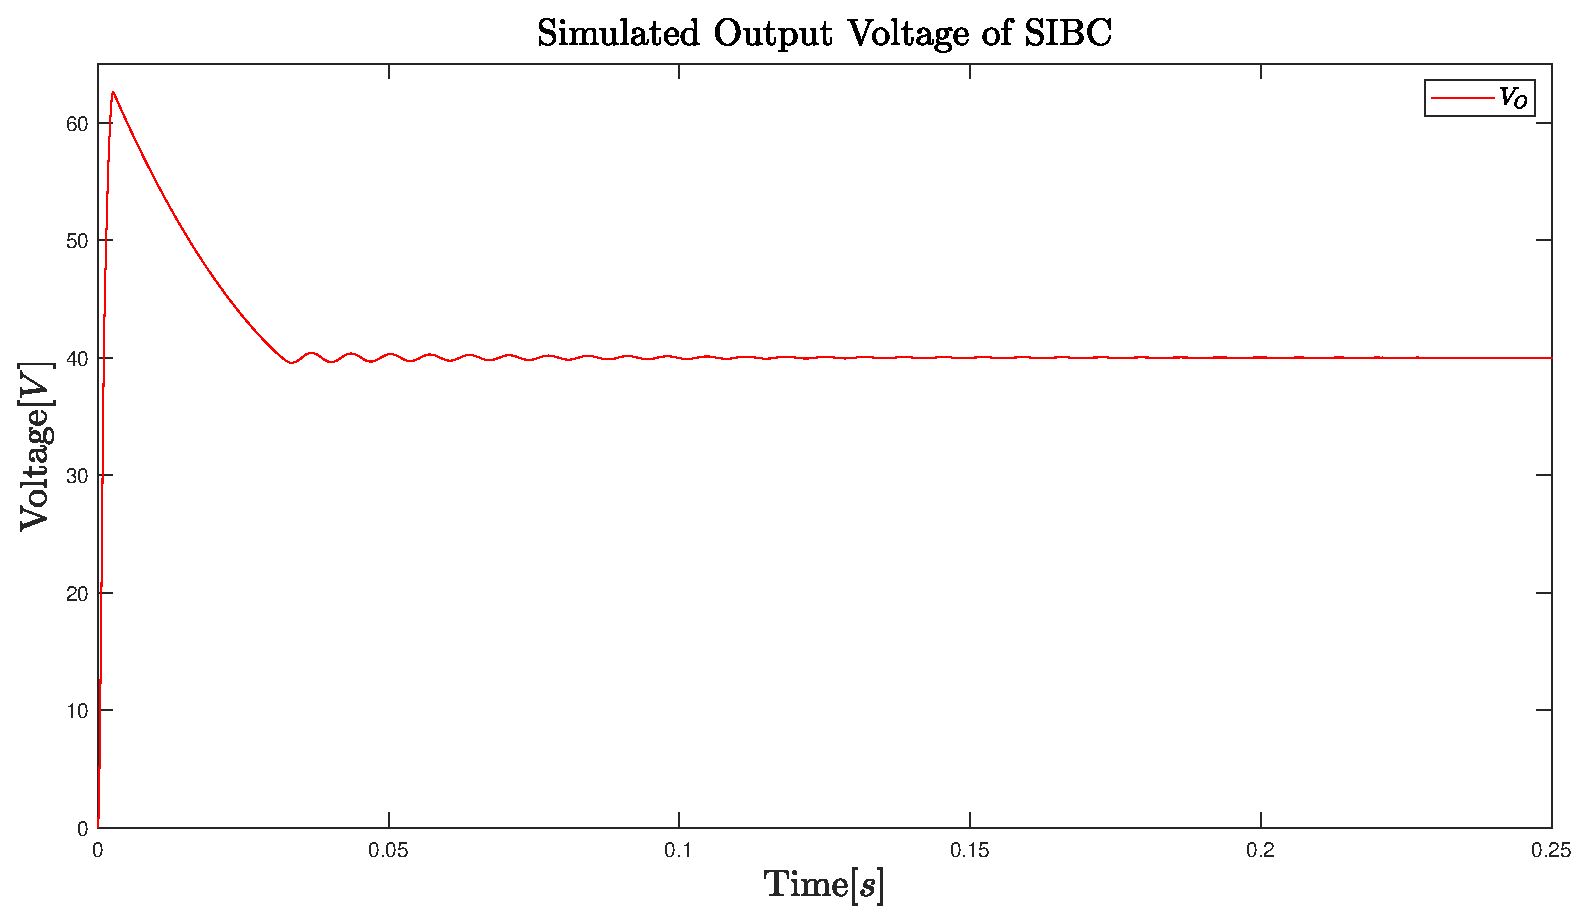
\includegraphics[width=0.8\textwidth]{figures/bSwitchedInductor/Simulation_SI.eps}
    \caption{Switched inductor boost output voltage}
	\label{fig:Simulation_SI}
\end{figure}
